In this work, we develop our generalized hierarchical Bayesian modeling framework that is able to capture the hierarchical structural relations and latent relations in the real-world recommendation scenarios. In our framework, we incorporate both user specific features and user actions into model learning so that more personalized recommendation results can be achieved. Furthermore, we present a variational inference algorithm for the HBayes framework to provide fast learning convergence.

In the following, we will describe how HBayes works by using apparel recommendation as an illustration scenario. Using a real-world example helps explain the hierarchy structural relations and latent variable conditional independence assumptions implied in HBayes. Please note that even we explain HBayes in apparel recommendation, the framework itself can be generalized into other recommendation scenarios with little modification. 

\subsection{Problem Statement}


\subsection{HBayes Framework}

We denote each event $i$ as a 4-tuple, i.e, ($\mathbf{x}_i, y_i, u, b$). $y_i$ is the binary label that indicates whether user $u$ has clicked the product from brand $b$ or not. $y_i$ is 1 means the click event happened. $\mathbf{x}_i$ represents the item and user features associated with event $i$. The conditional likelihood of event $i$ can be represented as follows:


\begin{equation}
p\big(y_i|\bm{x}_i,\bm{w}_b,\bm{w}_u \big)= \Big[\sigma\big(h_{i}\big)\Big]^{y_i} \cdot \Big[1-\sigma\big(h_{i}\big)\Big]^{1-y_i}
\end{equation}

\noindent where $\sigma(\cdot)$ is a logistic function, i.e. $\sigma(x)=(1+e^{-x})^{-1}$. $h_{i}\overset{\mathrm{def}}=\bm{x}_i^T(\bm{w}_b+\bm{w}_u)$. $\mathbf{x}^T$ is the vector transpose of $\mathbf{x}$. $\bm{w}_u$ and $\bm{w}_b$ represent the users and item's brand information encoded in HBayes. Therefore, the entire data likelihood becomes

\begin{equation}
\mathcal{L} = \prod_{i=1}^N p\big(y_i|\bm{x}_i,\bm{w}_b,\bm{w}_u \big)
\end{equation}



We use $\Theta$ to denote all model parameters:

\begin{equation}
\Theta \overset{\mathrm{def}}= \Big\{\{\bm{w}_u\}_{u=1}^U, \{\bm{w}_b\}_{b=1}^B, \{\bm{w}_s\}_{s=1}^S, \bm{w}, \bm{\theta}, \delta_u,\delta_b,\delta_s,\delta_w \Big\},
\end{equation}

\noindent and $\mathcal{H}$ to denote other hyper-parameters: $\mathcal{H} = \{\bm{\theta}, \alpha,\beta\}$.


The joint likelihood of the dataset $\mathcal{D}$, latent variable $\bm{Z}$ and the parameter $\Theta$ by given $\mathcal{H}$ could be written as follows:

\begin{align}
  p(\mathcal{D},\bm{Z},\Theta|\mathcal{H})= & \prod_{i=1}^N p(y_i|\bm{x}_i,\bm{w}_b,\bm{w}_u)  \\ 
  \cdot &  \prod_{b=1}^B p(\bm{w}_b|\bm{z}_b,\bm{w}_s,\delta_b) p(\bm{z}_{b}|\bm{\theta}) p(\bm{\theta}|\bm{\gamma}) p(\delta_b|\alpha,\beta) \\
  \cdot & \prod_{s=1}^S p(\bm{w}_s|\bm{w},\delta_s) p(\bm{w}|\delta_w)p(\delta_w|\alpha,\beta) p(\delta_s|\alpha,\beta) \\
   \cdot & \prod_{u}^U p(\bm{w}_u|\delta_u) p(\delta_u|\alpha,\beta) 
\label{joint_p}
\end{align}


\begin{figure}[htb]
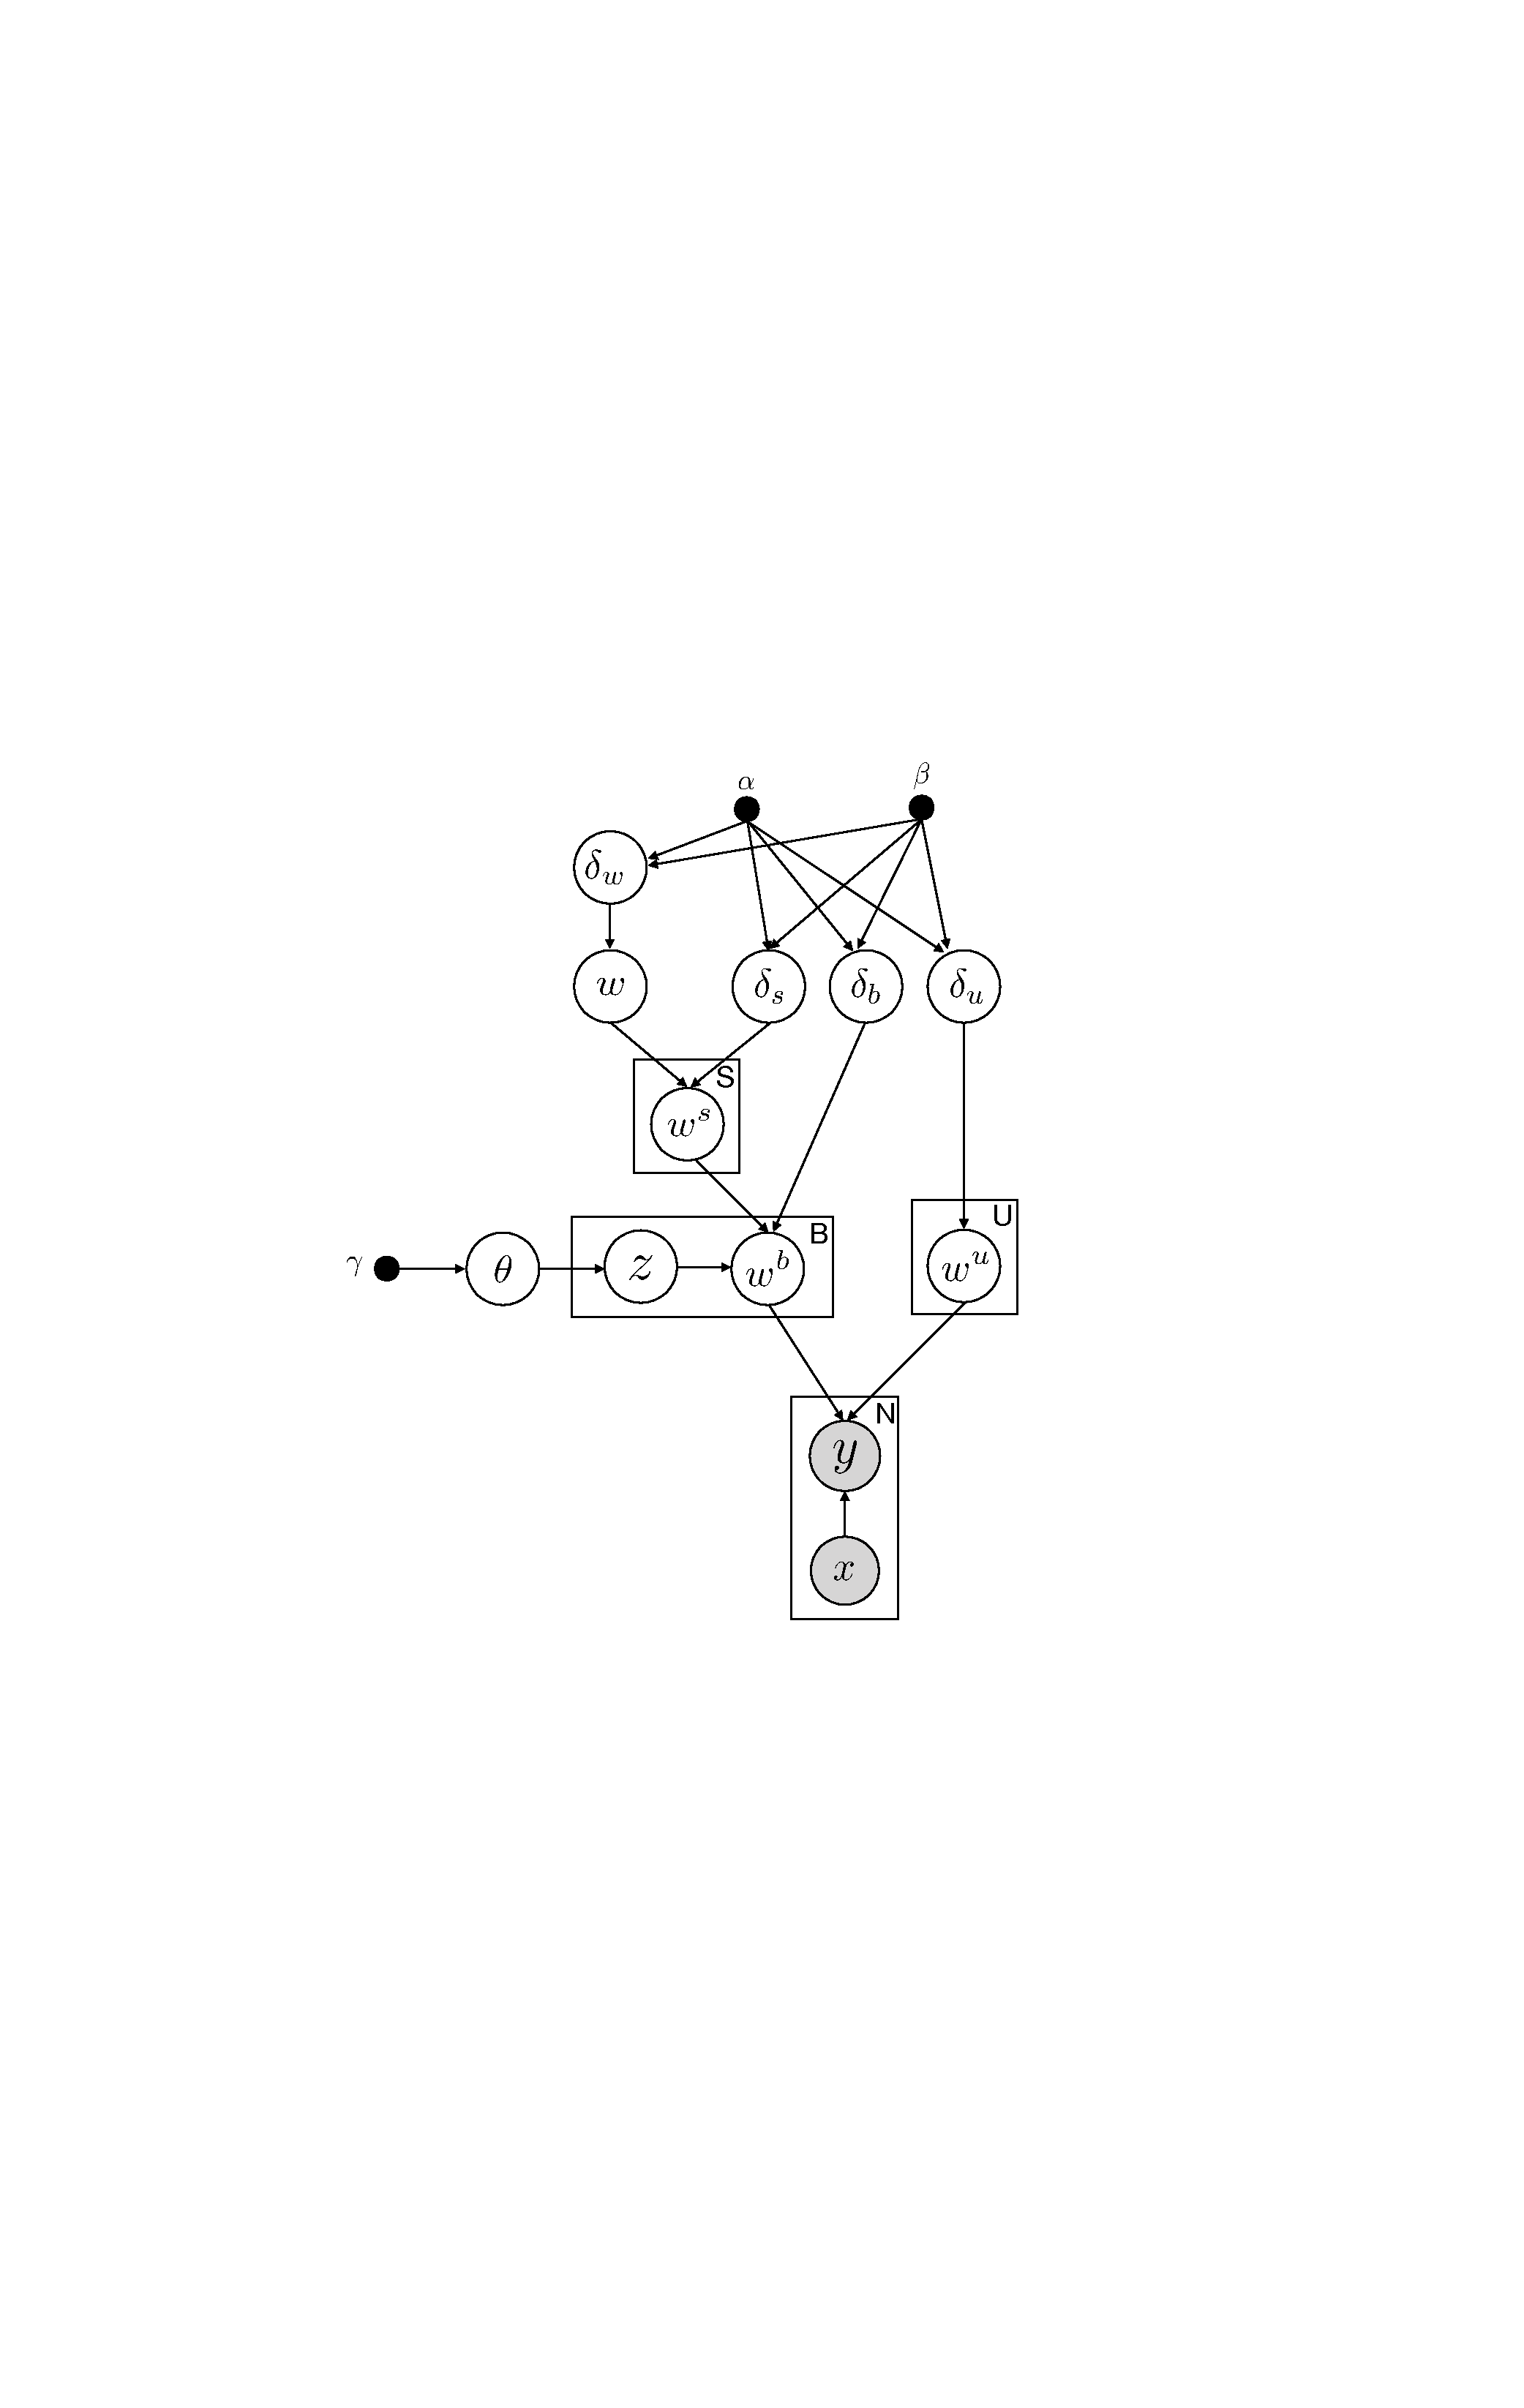
\includegraphics[width=0.8\linewidth]{fig/model}
\caption{Training time under different feature combinations on e-commerce recommendations}
\label{fig:train_time_cmp}
\end{figure}

\subsection{Optimization}

\subsubsection{Inference}

\begin{equation}
p(\bm{Z},\Theta|\mathcal{D},\mathcal{H}) = \frac{p(\mathcal{D},\bm{Z},\Theta|\mathcal{H})}{p(\mathcal{D}|\mathcal{H})}
\end{equation}

In this section, we apply variational Bayes to approximate the posterior distribution $p(\bm{Z},\Theta|\mathcal{D},\mathcal{H})$ with a variational distribution $q(\bm{Z},\Theta)$, by maximizing the variational free energy defined as:
\begin{equation}
\mathcal{L}(q)= \int_\Theta \sum_{\bm{Z}} q(\bm{Z},\Theta) \log\frac{p(\mathcal{D},\bm{Z},\Theta|\mathcal{H})}{q(\bm{Z},\Theta)}d\Theta
\end{equation}

\subsubsection{Sigmoid Approximation}

\begin{equation}
\sigma(h_{i}) \geq \sigma(\xi_{i})\exp\big\{\frac{1}{2}(h_{i}-\xi_{i})-\lambda_{i}(h_{i}^2-\xi_{i}^2)\big\}
\end{equation}

$$\lambda_{i}\overset{\mathrm{def}}=\frac{1}{2\xi_{i}}[\sigma(\xi_{i})-\frac{1}{2}]$$

\noindent where $\xi_{i}$ is a variational parameter. This lower bound is derived using the convex inequality. The similar problem was discussed in \cite{jaakkola1997variational,jordan1999introduction}.

\begin{align}
& \big[\sigma(h_{i})\big]^{y_i} \cdot  \big[1-\sigma(h_{i}) \big]^{1-y_i} \\
= & \exp\big\{ y_i h_i \big\} \sigma(-h_{i}) \\
\geq & \sigma(\xi_{i})\exp\big\{y_i h_{i}-\frac{1}{2}(h_{i}+\xi_{i})-\lambda_{i}(h_{i}^2-\xi_{i}^2)\big\}
\end{align}

% \begin{equation}
% \begin{split}
% \sigma(h_{i})^{y_i} \cdot & \big[1-\sigma(h_{i})  \big]^{1-y_i} \geq \\
%  & \sigma(\xi_{i})\exp\big\{y_i h_{i}-\frac{1}{2}(h_{i}+\xi_{i})-\lambda_{i}(h_{i}^2-\xi_{i}^2)\big\}
% \label{bound}
% \end{split}
% \end{equation}

\subsubsection{Learning}

\subsection{Prediction}

\subsection{Summary}